%%Part of the template, acmart is the ACM formatting as far as I'm aware

\documentclass[manuscript,screen,review]{acmart}
%%\begin{document} works like <html> </html> and wraps document
\begin{document}

%%Title, works like a variable, referenced with \maketitle later
\title{Context-Aware Sound Alerts}

%%Author information
\author{Dan Butcher}
\affiliation{%
  \institution{Colorado State University}
  \city{Fort Collins}
  \state{Colorado}
  \country{USA}}
\email{Dan.Butcher@colostate.edu}

\author{Elita Danilyuk}
\affiliation{%
  \institution{Colorado State University}
  \city{Fort Collins}
  \state{Colorado}
  \country{USA}}
\email{Elita.Danilyuk@colostate.edu}

\author{Zachariah Lamb}
\affiliation{%
  \institution{Colorado State University}
  \city{Fort Collins}
  \state{Colorado}
  \country{USA}}
\email{zplamb@colostate.edu}

\author{Zachary Lowe}
\affiliation{%
  \institution{Colorado State University}
  \city{Fort Collins}
  \state{Colorado}
  \country{USA}}
\email{zachary.lowe@colostate.edu}

%%Takes title information from above and inserts it into document
\maketitle
https://www.overleaf.com/project/6418d69fe6eafc07089377cd


\section{Introduction}
%%For the introduction, you need to have a strong introduction of what the project is about, and the motivation. Introduce the problem you are working on and the reason why is important. At this point, I expect citations of statements that are important.  

Although many human interactions with computers utilize senses such as vision and touch. Many technological developments have allowed and enabled the use of multiple senses to allow more natural and rich experiences across a range of the technology's abilities \cite{3411763.3441356}. Furthermore, senses can even form a sense of self and identity which further drives a person's embodied experience \cite{azanon2016multimodal}. Sound itself is used in our everyday lives to gain information about the environment around us \cite{1859799.1859808}. Thus, the realm of auditory interaction can be considered important. Notifications, regardless of medium, serve as a reminder that interaction is needed or as a response to an action taken. With respect to sound alerts, they are a significant part of how we interface with our machines. These help to guide users as they interact with their devices, and can even be leveraged to assist those with visual impairments \cite{10.1145/3232078.3232083}.

This project is important because effective notifications are beneficial to our productivity as opposed to silent interactions \cite{10.1145/2785830.2785852}, they improve the usability of our devices, and can even be lifesaving depending on the situation \cite{doi:10.1161/CIRCULATIONAHA.119.044126}. Context is defined by Dey \cite{dey2001understanding} as information used to characterize a person, place, or object relevant to the interaction between a user and an application. In order to use context and define a user and environment state, it would be ideal to have an adaptive context-aware system \cite{3274192.3274203}. As mentioned, contexts can be different depending on the context you want. For example, smartphone notifications could be looked at in the context of advertising services \cite{2851581.2892383}. We are looking at the context of sound alerts/notifications within the context of various background sounds. Because of this, we became interested in looking into the effectiveness of sound alerts after discussing how certain notifications can cut through a noisy environment more effectively than others.

We are looking to explore the relationship between humans and audio notifications with our research to better identify key attributes of sounds that are most effective in these different noisy environments. These notifications and their sound alerts are important, especially when considering mobile devices \cite{2493190.2493225} because they alert users about many things from emails to new messages and other events \cite{2628363.2628364, 2556288.2557189}. Because our devices have limited ways of communicating with us while our attention is diverted elsewhere, we look forward to using this project as an opportunity to find the common thread that makes certain notifications more noticeable and apparent than others.


\section{Related Works}
%%For the related works, at this point, make sure this is a story and not a summary paper by paper (the whole paper is a story). Checkpoint 1 expects at least 10 peer-reviewed papers cited. Checkpoint 2 expects at least 15 peer-reviewed papers cited.

Notifications, and the response individuals have to differing types of notifications, have important implications in the real world. This is because device notifications and alerts demand the user's attention, and as Mehrotra and Musolesi point out, this should be largely considered when sending alerts within different contexts within the real world \cite{10.1145/2750858.2807544}. Gallud and Tesoriero understood that notifications interrupt users and stop what they are doing \cite{10.1145/2786567.2793706}.  Although they studied sound and visual notifications, this paper will focus solely on alert sounds. Locken et al. devised another similar study in which the participant only had two cues to pay attention to. First was an ambient white noise sound that, when heard, the participant responded with an input key. Second, were visual cues in the form of LED displays. From this study, it was found that the participants learned and performed better over time and the visual cues distracted the participants from the audio cues \cite{10.1145/3119881.3119894}. Learning from this we have adjusted the counter-balancing design in our study to reduce the effect of the participant learning and we have also taken into consideration the number of visuals on the screen to reduce the number of distractions in order to solely focus on the notification and background sounds. 

In Yun (et. al) different audio-based notifications were studied on students taking part in online classes. The authors note a proclivity for some virtual students to be engaged in tasks other than learning during an online class. Audio notifications are an important way to get students' attention and convey important information in distance learning. Different types of sounds were rated in terms of pleasantness and resultant noticeability \cite{yun2022exploring}. The noticeability of an alert is an important factor, but some studies seek to understand how potentially jarring alerts affect our mental well-being. One can imagine that the most noticeable sound might also be frightening, startling, or emotionally abrasive. Payne examines a method of blending natural environmental sounds with traditional alerts in an effort to measure an effective alert that might be easy on the psyche \cite{payne2016ambient}. This attention to the emotional and physical result of an alert sound is interesting, however, in our experiment, we do not feel the alert sounds surpass a threshold of abusiveness in any way.

\subsection{User Attentiveness}
User attentiveness is important in human-computer interactions because users have a high number of notifications coming from their devices.
% Potentially ad a stat/citation here?
If the notification is considered important to the user, they want to be sure they notice and respond to it. A study by Li et. al focused on whether users' notification preferences on their smartphones would allow the predictability of their behaviors when they receive a notification \cite{10.1145/3478868}. The study found that users were less likely to respond to a notification if their preferences were rarely set to on, stating that users are more likely to be attentive and respond to notifications if they do receive the notification. Understanding that users' general preferences may have an effect on their attentiveness to a notification sound, our study has a demographic question asking users the average percentage during the day that their phone is on silent mode. The study by Li et. al also found that notifications were also less noticed and responded to in certain contexts; this further expresses the importance of understanding notification sound alerts given various background sounds/contexts in our study.

Users often have multiple notifications come through their devices on a daily bases. A study by Butz and Jung presented an approach of notifications that could provide notifications to one user and keep the other user undisturbed \cite{1040830.1040914}. This poses further thought on the context of the sound backgrounds and sound alert itself and whether multiple alerts would disrupt the users. Warnock and McGee-Lennon ran a study that showed that regardless of visual, auditory, or tactile cues, the disruption in the users' task was the same \cite{10.5555/2042118.2042173}. Mashhadi and Mathur importantly note that notifications do not all hold the same importance level to the user \cite{10.1145/2638728.2638759}. This study proceeds with the assumption that the notification sound goal is to distract the user from the task at hand. Similarly, a study by Iqbal and Horvits focused on notifications whose goal was to disrupt the user from their current tasks on their desktop computers \cite{10.1145/1718918.1718926}. Arfvidsson found shorter and congruent sounds perform better when subjects are listening to pick out the notifications against ambient background noises \cite{Arfvidsson21}. Although two notification sounds may be similar in harmonics, one may drastically outperform the other due to random variables such as an individual's general attentiveness or familiarity with the notification noise. This reinforces the importance of choosing a set of notification sounds that will provide clear results.

\subsection{Sound Traits}
The psychological traits of an individual and the implicated importance behind the notification can have a deep impact on the response time and how much of a disruption there may be on the given task. Gathering relative demographic data will be necessary to account for these inherently random variables. Not surprisingly, Singer \cite{Singer} showed that in order to be obviously noticeable against a background noise environment, the notification sounds should be played at a higher decibel volume; although, Singer did not find a specific range that is an ideal condition. It was also noted notification sounds in the higher frequency range performed better than those at lower frequencies though a larger sample size of sounds may prove this otherwise.

In another study, researchers focused on designing a sound identity for building brands and "corporate sound" and they focused fully on sound semantic descriptors, but were able to illustrate it to their users through communication tools to find appropriate sounds \cite{10.1145/2636879.2636896}.  Hanam, Tan, and Holmes found that they could even improve actionable alert sounds and rank them by finding patterns within static analysis alerts \cite{10.1145/2597073.2597100}. This study focused on not only finding actionable alert sounds but on alert identification techniques. On the other hand, to find the effectiveness of how disruptive a notification can be to working a task, Mehrota \cite{10.1145/2858036.2858566} found numerous confounding variables which may have a substantial influence on gathered results.

Garzonis, Bevan, and O'Neill conducted a study to find if auditory cues in the form of generic sounds, sounds tied to events, or speech were most effective at reducing response times in participants. From this study, it was discovered that there was little to no difference between generic sounds and event sounds, with the majority of the effect being tied to the specific event the sound is tied to or the user's previous experience with the generic sound. However, they found speech cues had a significant effect on the participants response time \cite{10.1145/1517744.1517793}. While our study will not include any speech cues, we have chosen the notification sounds used in our experiment to be generic and not tied to culturally significant sounds or cues.

%%For the methodology, make sure here you will describe what your experiment will do. In the methodology, you will also need to describe how the applications look (or will look like but assume it looks this way already). Either screenshots of the application, figures, or hand-drawing are ok at this point.

\section{Methodology}
Our experiment studied the noticeability of different alert sounds to human subjects when they are engaged in an activity in differing aural environments. This investigation was designed to study the aural interface between humans and the devices presenting notification sounds. After subjects completed their consent forms, the research moderator left the user in the room on their own, and let them know they can terminate the experiment at will. This allowed the reduction of potential vocal noise pollution and helped the possibility that the user would be more efficient in their task and ambiguity handling \cite{638249.638285}.

\begin{figure}[h]
  \centering
  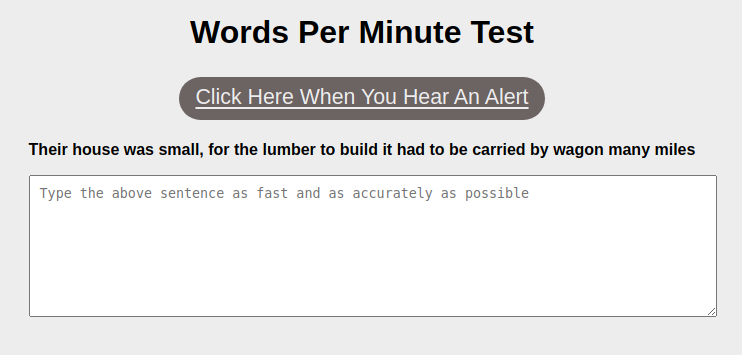
\includegraphics[scale=0.5]{images/wpm-test.png}
  \caption{The typing test interface.}
  \Description{A screenshot of our typing test with the action button to be pressed when an alert is heard.}
\end{figure}

The experiment was administered as a web application in a controlled environment. Before the presentation began, users were asked to fill out a demographics form to allow some insight on random variables like how often the user had their device notifications set to silent \cite{2702613.2732704}. The subjects were presented with a typing test, meant to occupy their attention. This strategy to distract the subject with a task was meant to simulate a realistic everyday situation in which a human is engaged in an activity and prompted for action by a sound when they may not be expecting it. We believe it was important to engage the participant’s attention to study the context of the notification. At the beginning of the typing test, we played an audio recording meant to simulate an acoustic environment. The environments were presented as different contexts, within which the notification sounds would be played. The sound level of each environment was held constant to allow the user to feel immersed in the experience \cite{raimbault2005urban}. The subjects were instructed to click a button when they heard a notification sound and then to resume typing which can be seen in Figure 1. The performance during the typing test was not important, with only the response time, combined with the notification and background noise pair, being collected as data. A series of different notification sounds were played at levels designed to be barely noticeable. The sounds were played a different times within each background sound/group because we were aware that scheduling alerts at different times would impact the subjects and their relative task \cite{1357054.1357070}. After a period of time, the typing test would conclude and the subject would then start a new instance of the typing test with a different background noise environment, repeating this phase for all aural environments.

This experiment had two independent variables, the three different sound alerts (Alert 1, Funk; Alert 2, Glass; Alert 2, Ping) and the environmental background sound (Airport, City, and Beach). These sounds were adopted by some quality attributes such as exciting, light, and eventful \cite{berglund2006tool}. The dependent variables were the sound alert recognition speed and missed notifications (if any). Each of the notification sounds were presented during a phase of the background sound environment and the order of the alerts was also randomized. In between each background/environmental sound phase, the user had a break with the screen showing a timer countdown until the next group of sounds begins. The experiment was delivered in a within-subject design. Each subject went through the same sound alerts and environmental sounds but both the order of the environmental phases and the order in which the alerts' sounds are played within each environmental phase were randomized. 

To avoid some random variables, the team kept several variables constant throughout each experiment. The first constant we kept was the system that the experiment was being run on, this is because we wanted to be sure that the user would not be interrupted multiple times during their task with other notifications that were not being tested \cite{1240624.1240730}. Next, we used over-ear headphones to block any potential unintended noise pollution \cite{3316782.3322739}. Another reason we decided on over-ear headphones was that speakers on a computer would take away the illusion of a real-world sound environment and a sound from a local site via the laptop would increase noise around the speaker and not the user themselves \cite{2658861.2658875}.

\section{Procedure}
Participation for the experiment was first solicited through Microsoft Teams and through in-person interactions with friends, coworkers, and fellow classmates. A Calendly scheduler was created prior to recruitment to facilitate sign-ups, and appointments were automatically created on a shared Google calendar. Two days prior to a given appointment an email was sent to participants reminding them of their time slot as well as providing further information regarding the location, time commitment, and expectations of the experiment.

\begin{figure}[h]
  \centering
  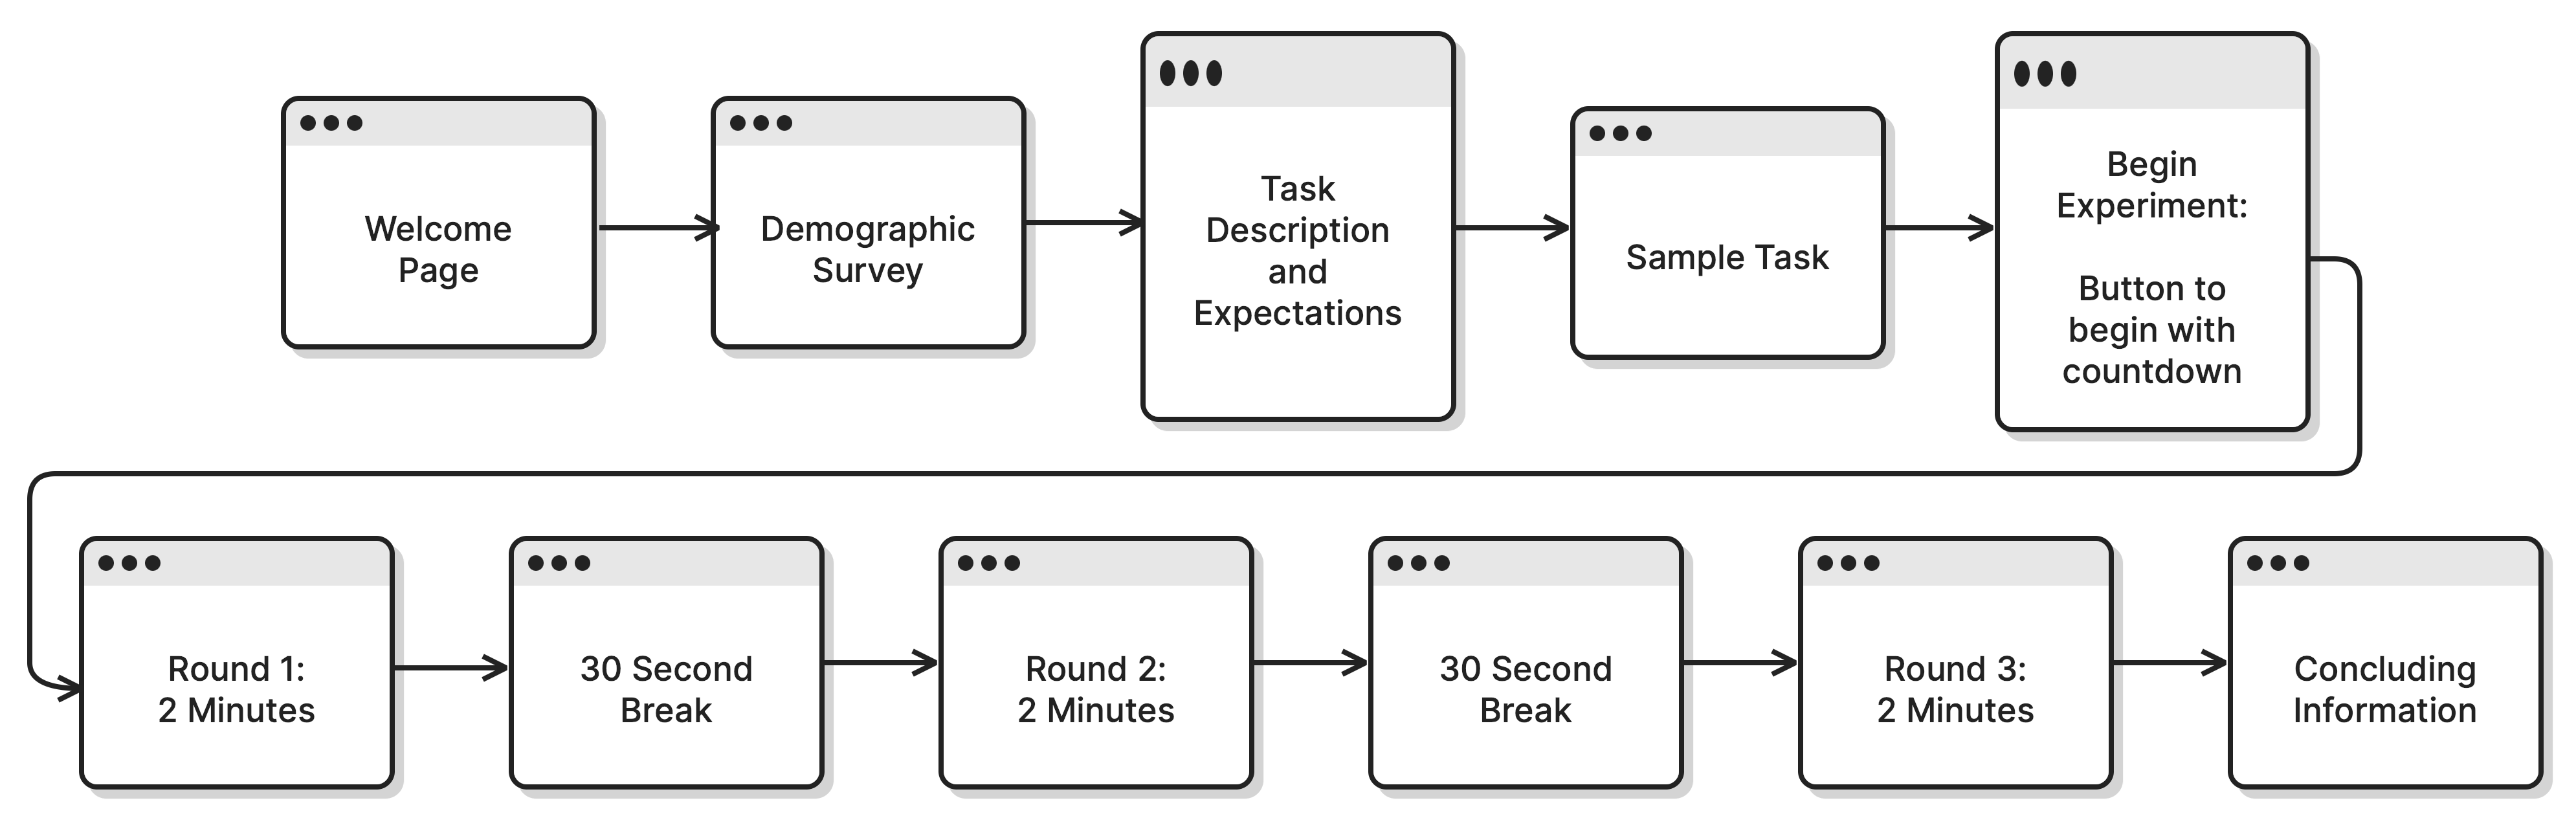
\includegraphics[width=\linewidth]{images/experiment-flow1.png}
  \caption{Our experiment design flow.}
  \Description{A flow diagram depicting our web application flow.}
\end{figure} 

Upon arrival, users were first asked to complete a consent form before beginning the experiment. Our experiment took place utilizing a React web application presented on a laptop provided to all subjects one at a time in a quiet room. There were a number of different pages displayed in the application to the subject during the experiment which can be visualized in the flow diagram of Figure 2. First, users began with a simple start screen explaining to them the context of the experiment and what was to be required of them. The instructions informed them that they are going to participate in a typing test and their performance will be measured. Next, a demographics survey was presented prompting the user to convey information about age, gender, preferred brand of phone, usage habits of their phone, and the amount of time they spend interacting with their device on average per day. After the demographics survey was completed the user then progressed at their own pace through a tutorial page. This page allowed the participant to interact with the typing window, the notification sounds, and the response button. They were reminded that the experiment is timed and were shown an example of the 30-second break timer that they would encounter during the experiment. They were asked to proceed to the experiment whenever they were ready to begin. 

Next, the independent variables were tested in the gamified typing test. They were given a prompt of text and told to type it in the provided text box. At the same time, various sounds to mimic remote work environments were played in the headphones. When they heard a sound alert, they were asked to stop typing and click a button to acknowledge the alert. This test continued for roughly three minutes, during which each of the three notifications were played in a randomized order. After each phase of a given environmental sound is complete, the user would then take a short 30-second break before being presented with the next environment. Concluding all environmental sound phases, the data was then collected and uploaded to a database, using their participant ID to identify it for later use. 

Lastly, the user was asked to participate in an exit survey using Google Forms that collected information about themselves and their experience. After the participant completed the final survey and exited, all surfaces including the laptop, headphones, and immediate area of the desk were sanitized. The experiment was then reset in preparation for the next participant.

\section{Data}
The data collected through our experimentation consisted primarily of reaction rates (hit rate) to the given alert stimulus. This not only measured reaction time but also allowed us to measure whether or not a notification was missed entirely by setting a hit threshold of 5000ms before flagging the alert as "missed". This data was collected by asking the participant to click a button on the screen in response to hearing an alert play. We measured the amount of time taken to click this button after the alert was initially played, and did not collect data on the words-per-minute (WPM) as this task was simply to prevent the participant from waiting for an alert to play. We also did not collect the data on WPM because people will often have difficulty returning to a task once they have been interrupted \cite{horvitz2001notification}. Similarly, once interrupted, users take a longer time to complete the previous task \cite{leiva2012back}. This can be further observed in the WPM during the experiment in the sense that once the user was interrupted it took a significant time for them to return to the WPM speed they were at before the interruption.

\begin{figure}[h]
  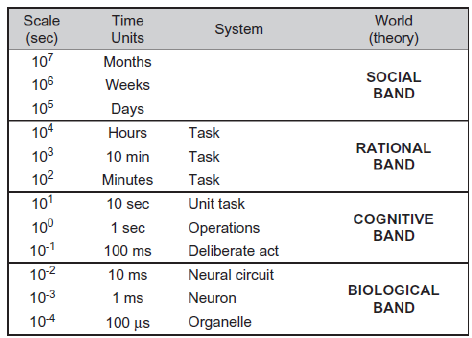
\includegraphics[scale=0.5]{images/Newells-Time-Scale.png}
  \caption{Newell's Time Scale of Human Action}
  \Description{Newell's time scale of human actions from United Theories of Cognition.}
\end{figure}

To gather the results and get hit rates and averages, we determined a 'hit threshold' of 5000 milliseconds (ms). This hit threshold was determined with Newell's Time Scale of Human Action \cite{newell1994unified}. For the threshold, we took the combination of biological and cognitive bands into consideration to give time for participants to register and respond to notification noises, Figure 3.



\section{Results}

\begin{figure}[h]
  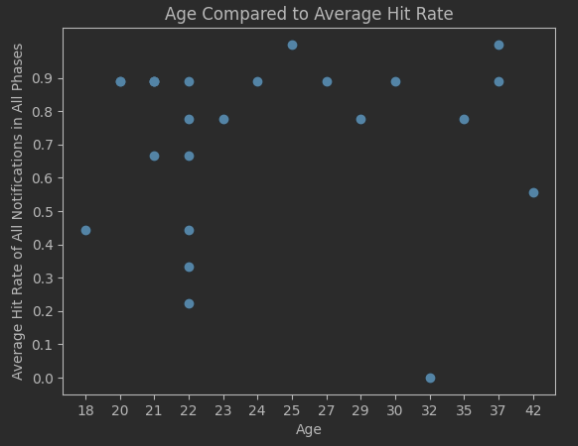
\includegraphics[scale=0.5]{images/age-performance-scatter.png}
  \caption{Age by Hit Rate}
  \Description{A scatter plot showing the average hit rates by age across all notifications, phases, and ages.}
\end{figure}

Of the data, we were able to not only examine the hit rates but also the age of a participant with their average hit rates. There does not seem to be a clear causation between the two, Figure 4. It can be seen in the same figure that at the hit rates around 90\% participants varied between the ages of 20 and 40. Interestingly enough, if you look at participants who were 22 years old, their average hit rates ranged between 20\% and 90\%.

\begin{figure}[h]
  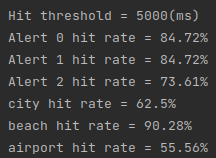
\includegraphics[scale=0.75]{images/hit-stats.png}
  \caption{Hit Stats}
  \Description{Hit rates per alert and background sound.}
\end{figure}

Figure 5 gives information related to hit rates given the hit threshold of 5000 ms. Overwhelmingly, the Beach background noise has the highest hit rate at 90.28\%. The background noise that presented the most challenging alert noticeability to the participants was the airport at 55.56\%. Although not quite as difficult as the airport, the city background noise was similarly low in terms of alert hit rate at 62.5\%. The alerts themselves presented less drastic differences in the effectiveness of noticeability, Figure 5. As mentioned previously our experiment Alert 0, titled "Funk" consisting of lower range frequencies, and Alert 1, titled "Glass" consisting of mid-range frequencies, both exhibited a hit rate of 84.72\%. Alert 2, titled "Ping" consisting of higher frequency tones produced the lowest hit rate at 73.61\%. Figure 6 further visualizes all of the average hit rates of the alerts and background noises compared to the hit rate threshold of 5000 ms.

\begin{figure}[h]
  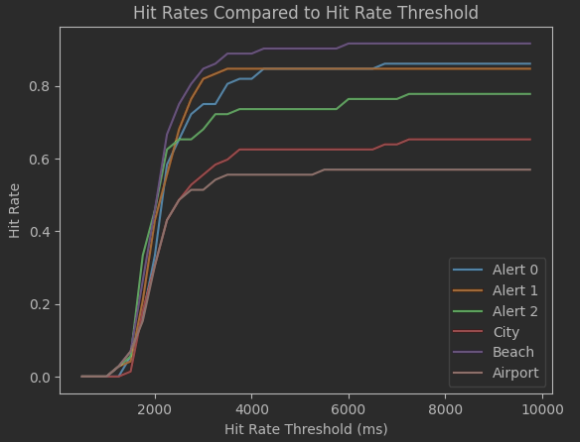
\includegraphics[scale=0.5]{images/hit-thresholds.png}
  \caption{Hit Rates Compared to the Hit Rate Threshold (5000 ms)}
  \Description{All average hit rates compared to the 5000-millisecond threshold.}
\end{figure}

\section{Conclusion}
Through our research and experimentation, we were able to identify that certain notifications were more recognizable across different sound contexts than others, but to a lesser degree than we had initially thought. In addition to this, we can conclude that certain ambient sound contexts themselves are more impairing to notification recognizability than others. When comparing the results of the Beach setting and the Airport setting, the difference in hit rate was significant. This is an important finding because a user may want to receive notifications with the same recognizability regardless of the background sounds and context. This could be related to a user's location or some other pattern, like time of day \cite{3406324.3417145}. We are not yet able to determine if the sound frequencies of these two background settings have any potential influence on this finding, but after concluding our experiments we also considered that the effectiveness of notifications on the Beach could have less to do with frequency and more to do with the lack of ambient conversation in the recording. Although we had not initially considered it, the human speech present in the Airport recording could have been more distracting to the listener whereas the Beach only has natural sounds without any dialogue. This isn't a factor that we can speak to given our current findings, but should be explored further should we continue our research.

In order to answer the new questions that this study has raised we have several new directions to move in terms of future research. Our next steps for this study would be to further investigate the characteristics of these sounds to tie possible frequency ranges to effectiveness and response time, and to also investigate the impact of human speech and how easily it can be ignored while performing a focused task. The Beach was the most successful soundscape in terms of hit rate. Although we are not yet able to draw a strong conclusion as to why, we have discovered a new area to move with our research and can consider this to be a success. Should we continue to further investigate the impact of human speech as a distraction to focused listening we may be able to gather more insight into what exactly made this phase of our experiment stand out. In order to do this we may want to conduct another study that omits any background environment that includes human speech but covers similar frequency ranges to determine whether or not the dialogue in the Airport was a confounding variable. This would require more in-depth study involving existing literature targeting human response to frequency ranges/a greater understanding of human hearing performance/calibrated experiments/things of this nature. A hearing test was not administered but would be useful for establishing a baseline to compare high success-rate alert frequencies against. Because a hearing test was omitted we cannot normalize user responses to existing hearing conditions and before we could design and perform a hearing evaluation we would need to learn more about what is needed to create a comprehensive and valid test that can adequately capture the hearing performance of the participant. This could potentially involve consulting with audiologists, researching existing hearing tests and protocols, and potentially designing our own custom hearing evaluation to fit the needs of our study.

Additionally, it could be beneficial to expand our research to investigate how different types of notifications, such as visual and haptic alerts, may perform in similar sound contexts. This could help us understand the full range of effectiveness of various notification modalities and identify potential areas of improvement for design and implementation. By understanding the impact of different modalities, we may be able to contribute further to the existing body of knowledge to support the creation of more effective and recognizable notifications.

Another potential direction to take our research could be to investigate the role of individual differences, such as age, gender, cultural background, and cognitive abilities, in the recognizability of notifications in various sound contexts. Understanding how these factors influence a person's ability to recognize and respond to notifications can help us develop more personalized and adaptive notification systems. Although we collected some demographic information from our respondents we did not attempt to tie these to any of our conclusions.

Finally, we could also potentially experiment with more specific real-world applications of alerts. By applying what we know know to practical and targeted situations we can increase the internal validity of our experiment and hopefully reduce noise and further identify specific attributes of sound that contribute directly to noticeability.

In conclusion, our study has provided valuable insights into the recognizability of notifications in different sound contexts and has raised important questions for future research. By further investigating the role of frequency ranges, human speech, individual differences, and real-world applications, we can continue to advance our understanding of effective notification design and contribute to the development of more efficient and user-friendly communication systems.


%% The next two lines define the bibliography style to be used, and
%% the bibliography file that is being referenced.
%% This portion shouldn't need changing, unless a different format is needed
%% or if we decide to rename the bibliography file
\bibliographystyle{ACM-Reference-Format}
\bibliography{CASAbib}

\appendix
%% Final data as csv is in this repo, final-data.csv

\end{document}